\documentclass[11pt]{preprint}

\setlength{\topmargin}{0mm} \setlength{\oddsidemargin}{0mm}
\setlength{\textwidth}{160mm} \setlength{\textheight}{215mm}

\usepackage{amssymb,amsmath,amscd,amsthm}
\usepackage{graphics}
\usepackage{tikz}

\def\enumb{\begin{enumerate}}
\def\enume{\end{enumerate}}
\def\itemb{\begin{itemize}}
\def\iteme{\end{itemize}}
\def\integers{\mathbb{Z}}

\def\multiset#1#2{\ensuremath{\left(\kern-.3em\left(\genfrac{}{}{0pt}{}{#1}{#2}\right)\kern-.3em\right)}}



\newtheorem{proposition}{Proposition}
\newtheorem{theorem}{Theorem}

\title{Discrete Mathematics, 2016 Fall- Worksheet 11}
\author{Instructor: Zsolt Pajor-Gyulai, CIMS}
\date{October 19, 2016}



\begin{document}

\maketitle

In all of the above problems explain your answer in full English sentences.

\enumb
\item Show algebraically that
\[
\frac{(2k+1)(k+1)k}{6}+(k+1)^2=\frac{[2(k+1)+1][(k+1)+1][k+1]}{6}.
\]

\begin{proof}
Pulling out $(k+1)$, it is enough to show
\[
\frac{(2k+1)k}{6}+k+1=\frac{[2(k+1)+1][(k+1)+1]}{6}
\]
On one hand
\[
LHS=\frac{2k^2+k+6k+6}{6}=\frac{2k^2+7k+6}{6},
\]
while
\[
RHS=\frac{(2k+3)(k+2)}{6}=\frac{2k^2+7k+6}{6}
\]
and we see that the two are equal.
\end{proof}
\item Let $n$ be a positive integer. Prove the following equations and inequalities by induction.
\enumb
\item $1+4+7+\dots+(3n-2)=\frac{n(3n-1)}{2}$.

\begin{proof}
Base case: When $n=1$, $1=\frac{1(3\cdot 1-1)}{2}=1$ holds.

Induction hypothesis: Suppose the result is true for $n=k$, i.e.
\[
1+4+7+\dots +(3k-2)=\frac{k(3k-1)}{2}.
\]

Induction step: Add $3(k+1)-2=3k+1$ to both sides to get
\[
1+4+7+\dots +(3(k+1)-2)=\frac{k(3k-1)}{2}+3k+1=\frac{3k^2+5k+2}{2}
\]
We can compute
\[
\frac{(k+1)(3(k+1)-1)}{2}=\frac{(k+1)(3k+2)}{2}=\frac{3k^2+5k+2}{2}
\]
which completes the proof of the induction step.
\end{proof}
\item $9+9\times 10+9\times 100+\dots+9\times 10^{n-1}=10^{n}-1$.

\begin{proof}
Base case $n=1$, we have that $9=10^0-1$.

Induction hypothesis: Assume that the claim is true for $n=k$, i. e., we have
\[
9+9\cdot 10+\dots+9\cdot 10^{k-1}=10^{k}-1
\]

Induction step: Add $9\cdot 10^k$ to both sides to get
\[
9+9\cdot 10+\dots+9\cdot 10^k=10^k-1+9\cdot 10^k=10\cdot 10^k-1=10^{k+1}-1
\]
\end{proof}
\item $1\cdot 1!+2\cdot 2!+\dots+n\cdot n!=(n+1)!-1$.
\begin{proof}
Base case $n=1$, we have $1\cdot 1!=(1+1)!-1$.

Induction hypothesis: Assume the claim holds for $n=k$, i.e.
\[
1\cdot 1!+\dots k\cdot k!=(k+1)!-1.
\]

Induction step: Add $(k+1)k!$ to both sides to get
\[
1\cdot 1!+\dots+(k+1)(k+1)!=(k+1)!-1+(k+1)(k+1)!=(k+2)(k+1)!-1=(k+2)!-1
\]
\end{proof}
\item $2^n\leq 2^{n+1}-2^{n-1}-1$.
\begin{proof}
Basis step $n=1$, we have $2=2^1\leq 2^{1+1}-2^{1-1}-1=2$.

Induction hypothesis: Assume the claim holds for $n=k$, i.e.
\[
2^k\leq 2^{k+1}-2^{k-1}-1
\]

Induction step: Multiply both sides of this by $2$ to get
\[
2^{k+1}\leq 2^{k+2}-2^k-2\leq 2^{k+2}-2^k-1.
\]
\end{proof}
\item $(1-\frac{1}{2})(1-\frac{1}{4})\cdot(1-\frac{1}{2^n})\geq\frac{1}{4}+\frac{1}{2^{n+1}}$.

\begin{proof}
Base case $n=1$, we have $\frac{1}{2}=(1-\frac{1}{2})\geq\frac{1}{4}+\frac{1}{2^2}=\frac{1}{2}$.

Induction hypothesis: Assume the claim holds for $n=k$, i.e.
\[
\left(1-\frac{1}{2}\right)\cdot\dots\cdot\left(1-\frac{1}{2^k}\right)\geq\frac{1}{4}+\frac{1}{2^{k+1}}
\]

Induction step: Multiply both sides by $\left(1-\frac{1}{2^{k+1}}\right)>0$ to get
\[
\left(1-\frac{1}{2}\right)\cdot\dots\cdot\left(1-\frac{1}{2^{k+1}}\right)\geq\left(\frac{1}{4}+\frac{1}{2^{k+1}}\right)\left(1-\frac{1}{2^{k+1}}\right)=\frac{1}{4}+\frac{1}{2^{k+1}}-\frac{1}{2^{k+3}}-\frac{1}{2^{2k+2}}
\]
\[
=\frac{1}{4}+\frac{1}{2^{k+2}}\left(2-\frac{1}{2}-\frac{1}{2^k}\right)=\frac{1}{4}+\frac{1}{2^{k+2}}\frac{2^{k+1}-2^{k-1}-1}{2^k}\geq\frac{1}{4}+\frac{1}{2^{k+2}}
\]
where we used the result of part (d).
\end{proof}
\enume

\item Suppose that a grid has $a+1$ vertical lines and $b+1$ horizontal lines. Prove by strong  induction that there are $\binom{a+b}{a}$ lattice paths from the lower left to the upper right corner.


\begin{center}
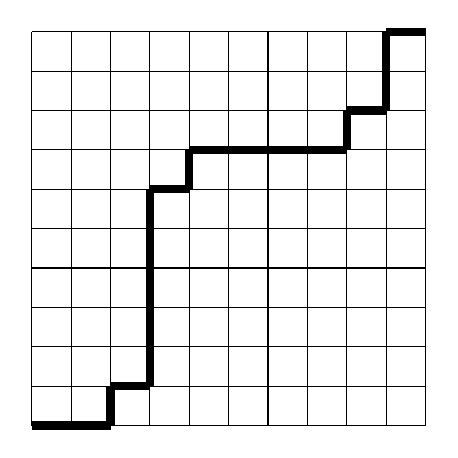
\begin{tikzpicture}[scale=0.5]
\foreach \i in {0,1,2,3,4,5,6,7,8,9,10}
	{
		\draw (\i,0) -- (\i,10);
	}
	
\foreach \i in {0,1,2,3,4,5,6,7,8,9,10}
	{
		\draw (0,\i) -- (10,\i);
	}
	
\draw[line width=3pt] (0,0) -- (2,0);
\draw[line width=3pt] (2,0) -- (2,1);
\draw[line width=3pt] (2,1) -- (3,1);
\draw[line width=3pt] (3,1) -- (3,6);
\draw[line width=3pt] (3,6) -- (4,6);
\draw[line width=3pt] (4,6) -- (4,7);
\draw[line width=3pt] (4,7) -- (8,7);
\draw[line width=3pt] (8,7) -- (8,8);
\draw[line width=3pt] (8,8) -- (9,8);
\draw[line width=3pt] (9,8) -- (9,10);
\draw[line width=3pt] (9,10) -- (10,10);

\end{tikzpicture}

Figure 2: Grid with $a=b=9$.
\end{center}

\begin{proof}
Base case: For $a=1$ and $b=1$, the grid is $1\times 1$ and the number of paths is two, which is also the value of $\binom{2}{1}$.

Strong induction hypothesis: Assume that the result is true for any $a<k_a$ or $b<k_b$.

Strong induction step: From the induction hypothesis, we know that there are $\binom{k_a-1+k_b}{k_a-1}$ paths from the lower left corner to the node to the left of the upper right corner. Similarly there is $\binom{k_a+k_b-1}{k_a}$ paths from the lower left corner to the node right below the upper right corner. Since the total number of paths from the lower left to the upper right corner is the sum of these two, we get that the total number is
\[
\binom{k_a-1+k_b}{k_a-1}+\binom{k_a+k_b-1}{k_a}=\binom{k_a+k_b}{k_a}
\]
by Pascal's identity. This finishes the proof.
\end{proof}


\item A flagpole is $n$ feet tall. On this pole, we display flags of the following types: red flags that are $1$ foot tall, blue flags that are $2$ feet tall, and green flags that are $2$ feet tall. The sum of the heights of the flags is exactly $n$ feet. Prove by induction that there are $\frac{2}{3}2^n+\frac{1}{3}(-1)^n$ ways to display the flags.

\begin{proof}
Basis case: Number of height one foot flags is exactly one (a red flag) which is also the value of $\frac{2}{3}2^1-\frac{1}{3}=\frac{4}{3}-\frac{1}{3}=1$.

Strong induction hypothesis: Assume that the claim is true for every flag of height $n<k$. 

Strong induction step: The number of flags of height $k$ is given by the number of flags of height $k-1$ (where we have no other choice but to add a red flag) plus twice the number of flags of height $k-2$ (when we can choose between a blue and a green flag to add). I.e. the total number of flags is
\[
\frac{2}{3}2^{k-1}+(-1)^{k-1}\frac{1}{3}+2\frac{2}{3}2^{k-2}+2(-1)^{k-2}\frac{1}{3}
\]
Assume for definiteness that $k$ is odd, the other case being similar. Then the above is
\[
\frac{2}{3}2^{k-1}+\frac{1}{3}+\frac{2}{3}2^{k-1}-\frac{2}{3}=\frac{2}{3}2^k-\frac{1}{3}.
\]
which is what we wanted to show.
\end{proof}


\item BONUS PROBLEM: Consider the following computer program.
\begin{verbatim}
function findMax(array, first, last){
  if (first==last) return array[first];
  mid = first+ (last-first)/2;
  a = findMax(array,first,mid); 
  b = findMax(array,mid+1,last);
  if (a<b) return b;
  return a;
}
\end{verbatim}
Here \verb array ~is an array of integers. All other variables are integers. We assume that \verb first ~and \verb last ~are between $1$ and the number of elements in \verb array ~and that \verb first $\leq$ \verb last . Note that if \verb last-first ~is odd, then (\verb last-first )/2 is rounded down to the nearest integer.

The purpose of this program is to find the largest value in the array between two indices; that is, it should return the largest value of
\begin{verbatim}
 array[first],array[first+1],...,array[last].
 \end{verbatim}
 Prove that this program fulfills this task.
\enume
\end{document}